\documentclass[main.tex]{subfiles}

\begin{document}
\section{Numerical Studies}
In this section we compare RgPCC with LASSO penalty to conventional logistic regression. We first summarize how our simulated data was created and then discuss the results of the methods mentioned previously. We will consider a variety of sample sizes, dimensions and sparsities in $\bgamma$ and compare error rates in $\p, \bbeta, \bgamma$ and classification. We will also vary which components of $\bgamma$ are nonzero. Again, please note that $p$ is the number of predictors while $\p$ is a vector of probabilities.

\begin{figure}[H]
	\begin{tabular}{l l l} \hline
		$p$ & $N$ & $\bgamma$ sparsity \\ \hline
		\rowcolor{LightCyan}
		12 & 100, 200 & 1, 3, 5 \\
		50 & 100, 200 & 1, 3 \\
		\rowcolor{LightCyan}
		80 & 100, 200 & 1 \\ \hline
	\end{tabular}
	\caption{Parameters of data creation.}
	\label{figure:params}
\end{figure}

The convergence of our algorithm is based on the tolerance of $\varepsilon = 0.1$, which means we will terminate our Newton-Ralphson method when $$\varepsilon^{(k)} = \frac{||\bbeta^{(k)} - \bbeta^{(k+1)}||}{||\bbeta^{(k)}||} < 0.1.$$

\subsection{Creation of Simulated Data}
Let $\gls{X}$ be our design matrix where each row of $\gls{X}$ is independently generated from $N(0, \Sigma)$ where $\Sigma_{ij} = \rho^{|i - j|}$ with $\rho = 0.8$.

To generate our response data, let $\mu = \gls{X} \bbeta^* = \gls{U} \bgamma^*$ where $\bgamma^* = \gls{D} \gls{V}^T \bbeta^*$. Then the classes $\y$ come from a Bernoulli distribution with parameter $\p = \frac{\text{exp}(\U \bgamma^*)}{1 + \text{exp}(\U \bgamma^*)} = \frac{\text{exp}(\mu)}{1 + \text{exp}(\mu)}$. Therefore the response data is dependent on $\bgamma^*$ and the data $\gls{X}$. We make a variety of choices for $\bgamma^*$ (denoted just as $\bgamma$ below) which have varying amounts of sparsity and created varying levels of linear separability.

\subsection{Performance of RgPCC on Simulated Data}
Here we fit RgPCC, logistic regression and PC logistic regression to our simulated data. To test the quality of the fit, we see how well our models predict the true probability vector $\p$ (the parameter of the Bernoulli distribution above) over a test set of size $5N$. We measure the accuracy of our predicted \gls{probhat} using the 1-norm, 2-norm and EGKL. These are defined as follows:

\begin{align*}
	\text{1-norm error} & \hspace{1cm} \sum_{i = 1}^N |\widehat{\p}_i - \p_i| \\
	\text{2-norm error} & \hspace{1cm} \sum_{i = 1}^N (\widehat{\p}_i - \p_i)^2 \\
	\text{EGKL loss} & \hspace{1cm} \sum_{i = 1}^N \p_i \log \left ( \frac{\p_i}{\widehat{\p}_i} \right )
\end{align*}
We fit the models using samples of size $N$ for dimension $p$ from Figure \ref{figure:params}. We also vary the nonzero components of the true $\bgamma$. We neglect the case where $N < p$, although there are no theoretical issues in this case and will be covered in further research.

We use the following values for the true $\bgamma$:
\begin{figure}[H]
	\begin{tabular}{l}
		$\bgamma_1 = (25, 0, \ldots , 0)$ \\
		$\bgamma_2 = (20, 10, 10, 0, \ldots , 0)$ \\
		$\bgamma_3 = (15, 10, 5, 5, 3, 0, \ldots , 0)$\\
		$\bgamma_1' = (0, 0, 0, 0, 0, 25, 0, \ldots , 0)$ \\
		$\bgamma_2' = (0, 0, 0, 0, 0,  20, 10, 10, 0, \ldots , 0)$ \\
		$\bgamma_3' = (0, 0, 0, 0, 0,  15, 10, 5, 5, 3, 0, \ldots , 0)$
	\end{tabular}
\end{figure}

Below we show only a few cases of all the tests. The rest of the results are present in the last section but have the same conclusion as the one presented here.
\begin{figure}[H]
    \centering
    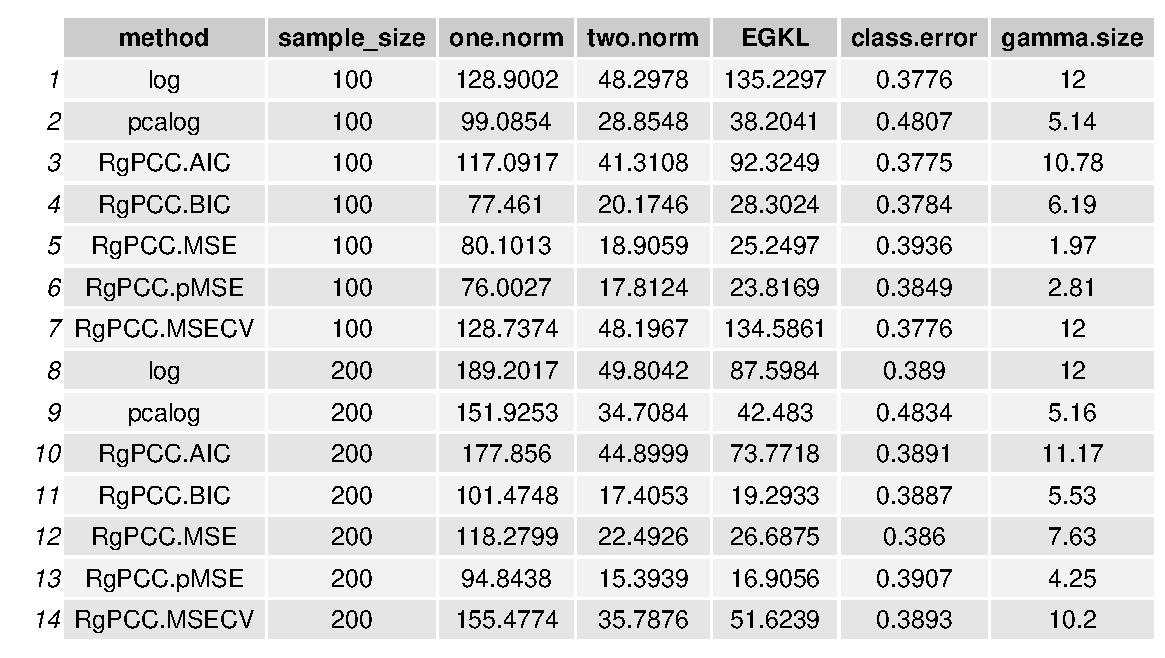
\includegraphics[width =  \textwidth]{simulated/(sparsity3-nonlead,12)_metrics.pdf}
    \caption{Simulated results for RgPCC with parameters $\bgamma_2'$ and $p = 12$.}
    \label{fig:simulated2-12}
\end{figure}

\begin{figure}[H]
	\centering
    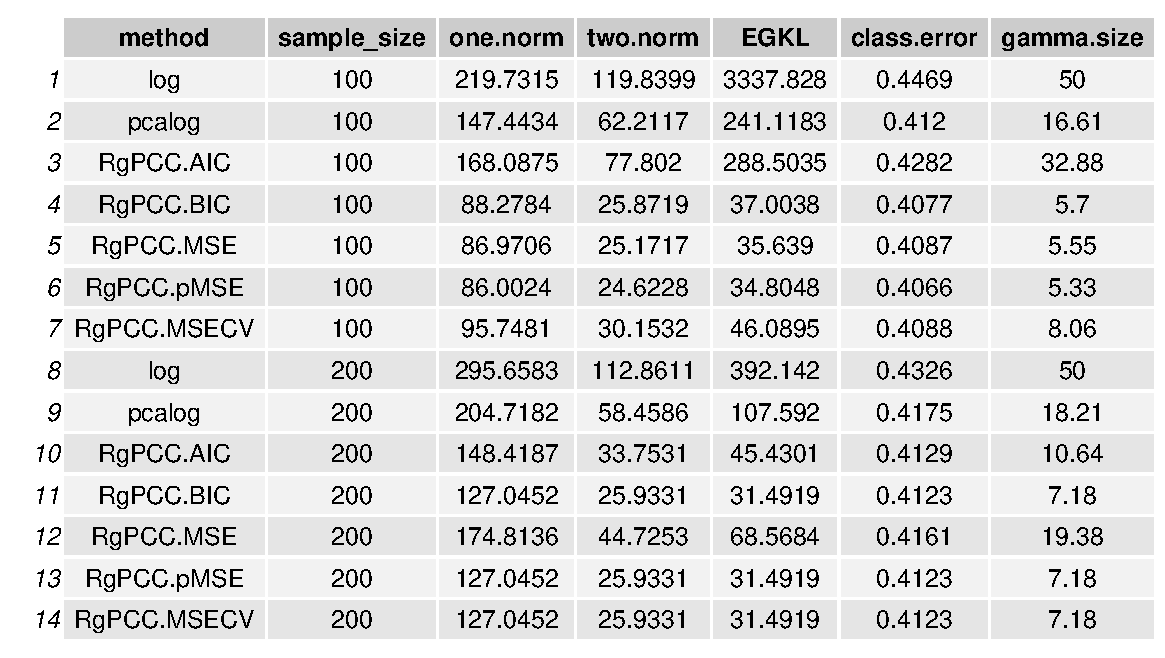
\includegraphics[width =  \textwidth]{simulated/(sparsity3-nonlead,50)_metrics.pdf}
    \caption{Simulated results for RgPCC with parameters $\bgamma_2'$ and $p = 50$.}
    \label{fig:simulated2-50}
\end{figure}

Overall, we see that RgPCC provides a slight improvement in the testing classification error compared to logistic regression and PC logistic regression. However, the real improvement in in the accuracy of our prediction of $\p$.

Overall, we can see that RgPCC provides slight improvements in the classification error to logistic regression and principal component logistic regression when the true $\bgamma$ is nonzero in the leading principal components. However, when the nonzero components of $\bgamma$ are not the leading principal components we see a significant different between principal component logistic regression and our other methods.

% \begin{table}[H]
% % (N, p) = (100, 500)
% \begin{subtable}{0.5 \linewidth}
% \begin{tabular}{l|lll} \hline
% 	 & $\bgamma_1$ & $\bgamma_2$ & $\bgamma_3$ \\ \hline
% 	\rowcolor{LightCyan}
% 	RgPCC AIC &&& \\
% 	RgPCC BIC &&&  \\
% 	\rowcolor{LightCyan}
% 	Logistic &&& \\
% 	PC Logistic &&& \\ \hline
% \end{tabular}
% \caption{$N = 100$}
% \end{subtable}%
% % (N, p) = (100, 500)
% \begin{subtable}{0.5 \linewidth}
% \begin{tabular}{l|lll} \hline
% 	 & $\bgamma_1$ & $\bgamma_2$ & $\bgamma_3$ \\ \hline
% 	\rowcolor{LightCyan}
% 	RgPCC AIC &&& \\
% 	RgPCC BIC &&& \\
% 	\rowcolor{LightCyan}
% 	Logistic &&& \\
% 	PC Logistic &&& \\ \hline
% \end{tabular}
% \caption{$N = 200$}
% \end{subtable}%
% \caption{p = 100}
% \end{table}

We can see that the testing error for $\p$ is improved with RgPCC by at least a factor of 4 in each case. RgPCC avoids overfitting the data as much as logistic regression does. In particular, there is drastic improvement in classification when $\bgamma^*$ is very sparse (that is for $\bgamma_1$). Similar results occur when $N = 200$ but are left in the table and results section.

We also run a few examples for higher dimensional data. Our method should excel in this via its use of principal components and sparsity in $\bgamma$.

where

\begin{figure}[H]
	\begin{tabular}{l}
		$\bgamma_1 = (25, 0, 0, 0, 0, 0, \ldots , 0)$ \\
		$\bgamma_2 = (10, 5, 5, 0, 0, 0, \ldots , 0)$
	\end{tabular}
\end{figure}

Here we see similar results as in the low dimensional case. At this point, we know that RgPCC performs better, if no just as well, as logistic regression does. However, there are still many aspect of the method we wish to study.

\subsection{Performance of RgPCC on Realworld Data}

In this section we apply four real datasets to compare the prediction performance of RgPCC with conventional binary classification methods. We look at the following data sets.
\begin{itemize}
    \item Divorce Predictors (170 instances, 54 predictors, binary response)
    \item Cryotherapy (90 instances, 7 predictors, binary response)
    \item Audit (777 instances, 18 predictors, binary response)
    \item Ecoli (336 instances, 8 predictors, binary response)
\end{itemize}

We will compare the methods RgPCC, logistic, PCA logistic and ridge regression. We will tune RgPCC by AIC and BIC. Thus we will compare a total of five different methods. 

To compare the performance of our binary classification methods based on the error of each fold of 5-fold cross validation. We then perform Tukey's multiple pairwise comparison to test if the methods differ significantly or not.

The following is a summary of the error results, more can be found in the section 6.

\begin{figure}[H]
	\begin{tabular}{l l l l l l} \hline
    & RgPCC AIC & RgPCC BIC & Logistic & PC Logistic & Ridge \\ \hline
    \rowcolor{LightCyan}
    Divorce & 0.023529 & 0.023529 & 0.058823 & 0.035294 & 0.023529\\
    Cryo & 0.12222 & 0.12222 & 0.12222         &  0.5 & 0.14444 \\
    \rowcolor{LightCyan}
    Audit & 0.033548 & 0.030967 & 0.034838    & 0.18193 & 0.04129\\
    Ecoli & 0.041666 & 0.038690 & 0.041666  & 0.053571 & 0.044642\\ \hline
	\end{tabular}
	\caption{The mean classification errors over each of the 5 folds.}
\end{figure}

When running the Tukey's multiple pairwise comparisons we noticed that in most cases the difference in the errors was insignificantly different with $p$-values around $0.99 \geq \alpha = 0.05$. However, there were a few cases in which PC logistic was significantly different than all the other methods (Audit data and Cryotherapy). This data is given below.

\begin{figure}[H]
    \centering
    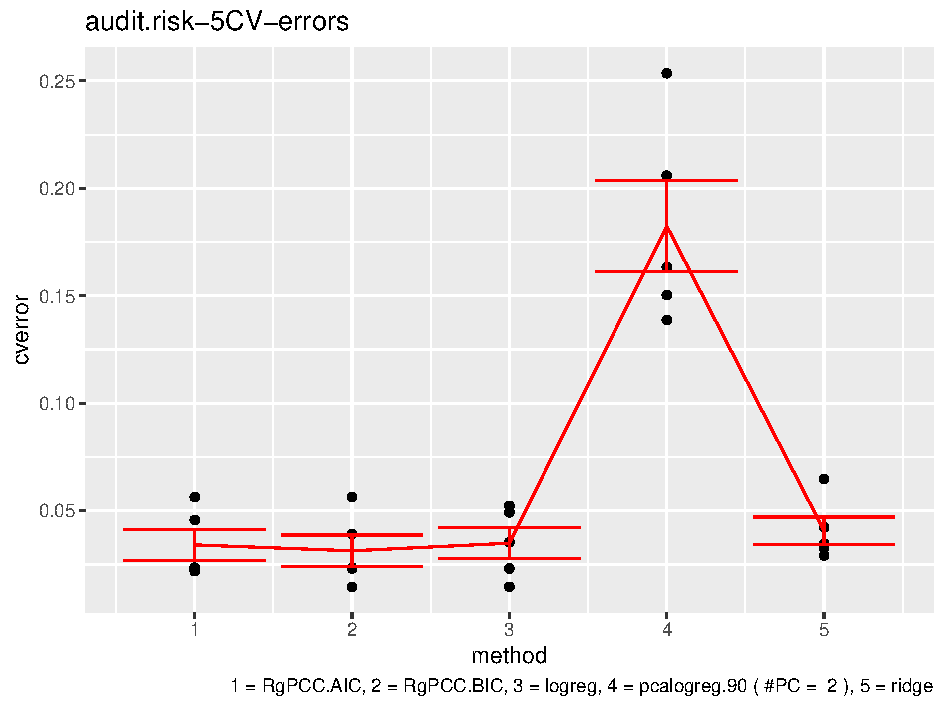
\includegraphics[width =  0.49\textwidth]{realworld/audit.risk-5CV-errors graph.pdf}
    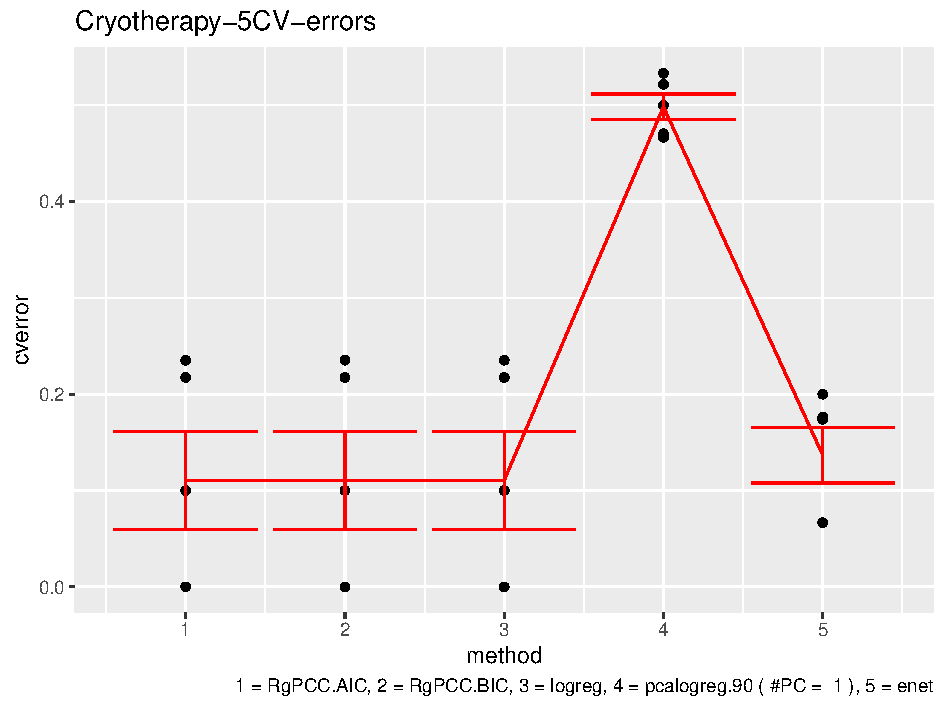
\includegraphics[width =  0.49\textwidth]{realworld/Cryotherapy-5CV-errors graph.pdf}
    \label{fig:my_label}
\end{figure}

Thus, in terms of classification error RgPCC is comparable to logistic and ridge regression in application settings.
\end{document}